\documentclass{article}
\usepackage{setspace}
\usepackage[utf8]{inputenc}
\usepackage{natbib}
\usepackage{url}
\usepackage{indentfirst} 
\usepackage{hyperref}
\usepackage{xcolor}
\usepackage{float}
\usepackage{booktabs}
\usepackage{longtable}
\usepackage{array}
\usepackage{multirow}
\usepackage{wrapfig}
\usepackage{float}
\usepackage{colortbl}
\usepackage{pdflscape}
\usepackage{tabu}
\usepackage{threeparttable}
\usepackage{threeparttablex}
\usepackage[normalem]{ulem}
\usepackage[utf8]{inputenc}
\usepackage{makecell}
\usepackage{xcolor}

\usepackage{graphicx}
\graphicspath{ {figures/} }

\title{Constructing Optimal MLB Teams with Linear Programming}
\author{Nathan Schor}
\date{August 28, 2022}

\doublespacing
\begin{document}

\providecommand{\keywords}[1]
{
  \small	
  \textbf{\textit{Keywords---}} #1
}

\maketitle
\begin{abstract}
Major League Baseball teams face trade-offs in assembling talented rosters without overspending. Teams need to make difficult choices about which players to roster, how many players to keep at each position, and how much to pay those players. This paper provides insights into managing these trade-offs thorough setting up a constrained optimization problem that seeks to maximize total team performance, subject to player salary and position constraints. 
\end{abstract}
\keywords{MLB, Constrained Optimization, Roster Construction}
\newpage
\tableofcontents
\newpage
\section{Introduction}

The purpose of this research is to investigate the relationship between salary and team performance in Major League Baseball (MLB). We do this by looking at actual outcomes for MLB teams in 2021 and compare those results to optimal rosters constructed via linear programming. Our goal is to analyze the gap between current team performance and their potential optimal performance. 

We begin with 2021 salary data for each MLB team from \cite{Brown2021}. This data is supplemented with each player's 2021 salary, team, position, and JEFFBAGWELL (our performance metric, abbreviated JB). JB stands for \textbf{J}oint \textbf{E}stimate \textbf{F}eaturing \textbf{F}anGraphs and \textbf{B}-R \textbf{A}ggregated to \textbf{G}enerate \textbf{W}ar, \textbf{E}qually \textbf{L}eveling \textbf{L}ists and is provided by \cite{JB}. WAR is a metric that quantifies each player's value in terms of how many wins they provide \cite{WAR}. Next, we seek to maximize JB for each of the 30 teams subject to salary and player position constraints, and visualize the results. Lastly, we discuss the implications of the gap between teams' current roster and their optimal roster.

\section{Literature Review}

The relationship between spending and performance is a topic of discourse among both casual fans and diehard fans, such as members of the SABR\footnote{SABR is the Society for American Baseball Research, an organization dedicated to discovering objective baseball knowledge \url{https://sabr.org/}} baseball community. The book \emph{Moneyball} by \cite{Moneyball} launched the baseball analytics revolution. One example of using linear programming in baseball is \cite{McIntyre2016}. Another example of linear programming in baseball is \cite{Adler99baseball}. An instance of linear programming in other sports is \cite{Aramouni2021}.

\section{Methodology/Data}

\subsection{Data Cleaning}

To clean the player dataset, we first assign positions to each player. A player's position is recorded as the position they played most frequently during the season (if they played two positions an equal amount of times, their position was randomly assigned to one of the two positions). Players with a \$0 salary or a missing salary are removed. A pitcher is classified as a Starting Pitcher (SP) if $\geq$ 50\% of their appearances were as a starter, and otherwise are classified as a Relief Pitcher (RP). Furthermore, First Basemen (1B), Second Basemen (2B), Third Basemen (3B), and Shortstops (SS) are classified as Infielders (IF). Left Fielders (LF), Center Fielders (CF), and Right Fielders (RF) are classified as Outfielders (OF). Catchers (C) and Designated Hitters (DH) are left as their own individual categories. 

\subsection{Salary and JEFFBAGWELL by Position}

Baseball teams need to make important decisions about which players to have on their team, and how much to pay them. An interesting aspect is that each position is not equally valuable to creating a winning team, and, consequently, players at different positions have varying salaries (controlling for skill level). 

In Figure \ref{fig:salary_position_boxplot}, we see how salary varies by position. The median salary for a Starting Pitcher is around \$5,000,000 while the median salary for a Relief Pitcher is closer to \$1,000,000. The salary distributions also vary drastically within infield and outfield positions. Starting Pitchers and Relief Pitchers also have the largest number of outliers.

\begin{figure}[H]
\caption{Boxplot of Salary (for Players with Salary $> \$0$) by Position}
\label{fig:salary_position_boxplot}
\centering
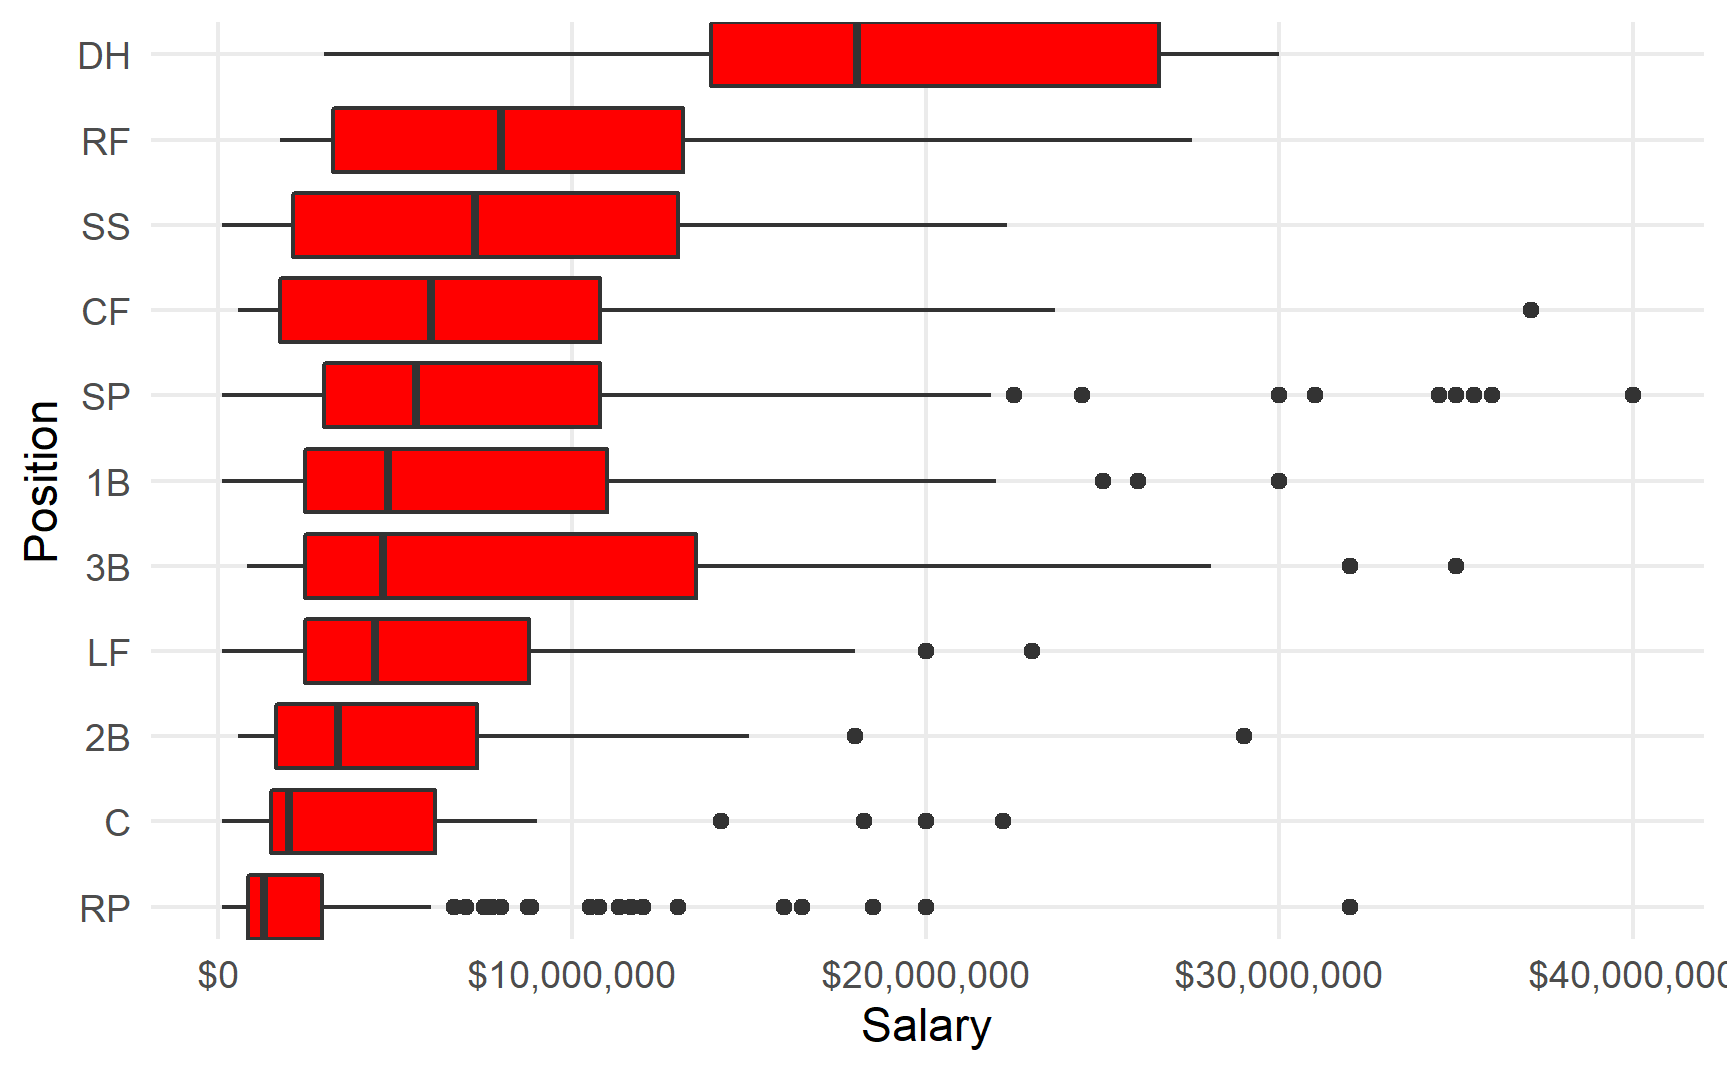
\includegraphics[width=0.7\paperwidth, scale=1.25]{salary_position_boxplots.png}
\end{figure}

It is interesting to compare this with Figure \ref{fig:war_position_boxplot}. C and RP have the lowest median values in both. However, IF and OF positions are much closer together in the JB plot. This suggests a potential discrepancy between how much players are valued and how much they are paid--if players were perfectly paid according to their value, we would expect the position ordering on the y-axis of the two graphs to be identical.  

\begin{figure}[H]
\caption{Boxplot of JEFFBAGWELL (for Players with Salary $> \$0$) by Position}
\label{fig:war_position_boxplot}
\centering
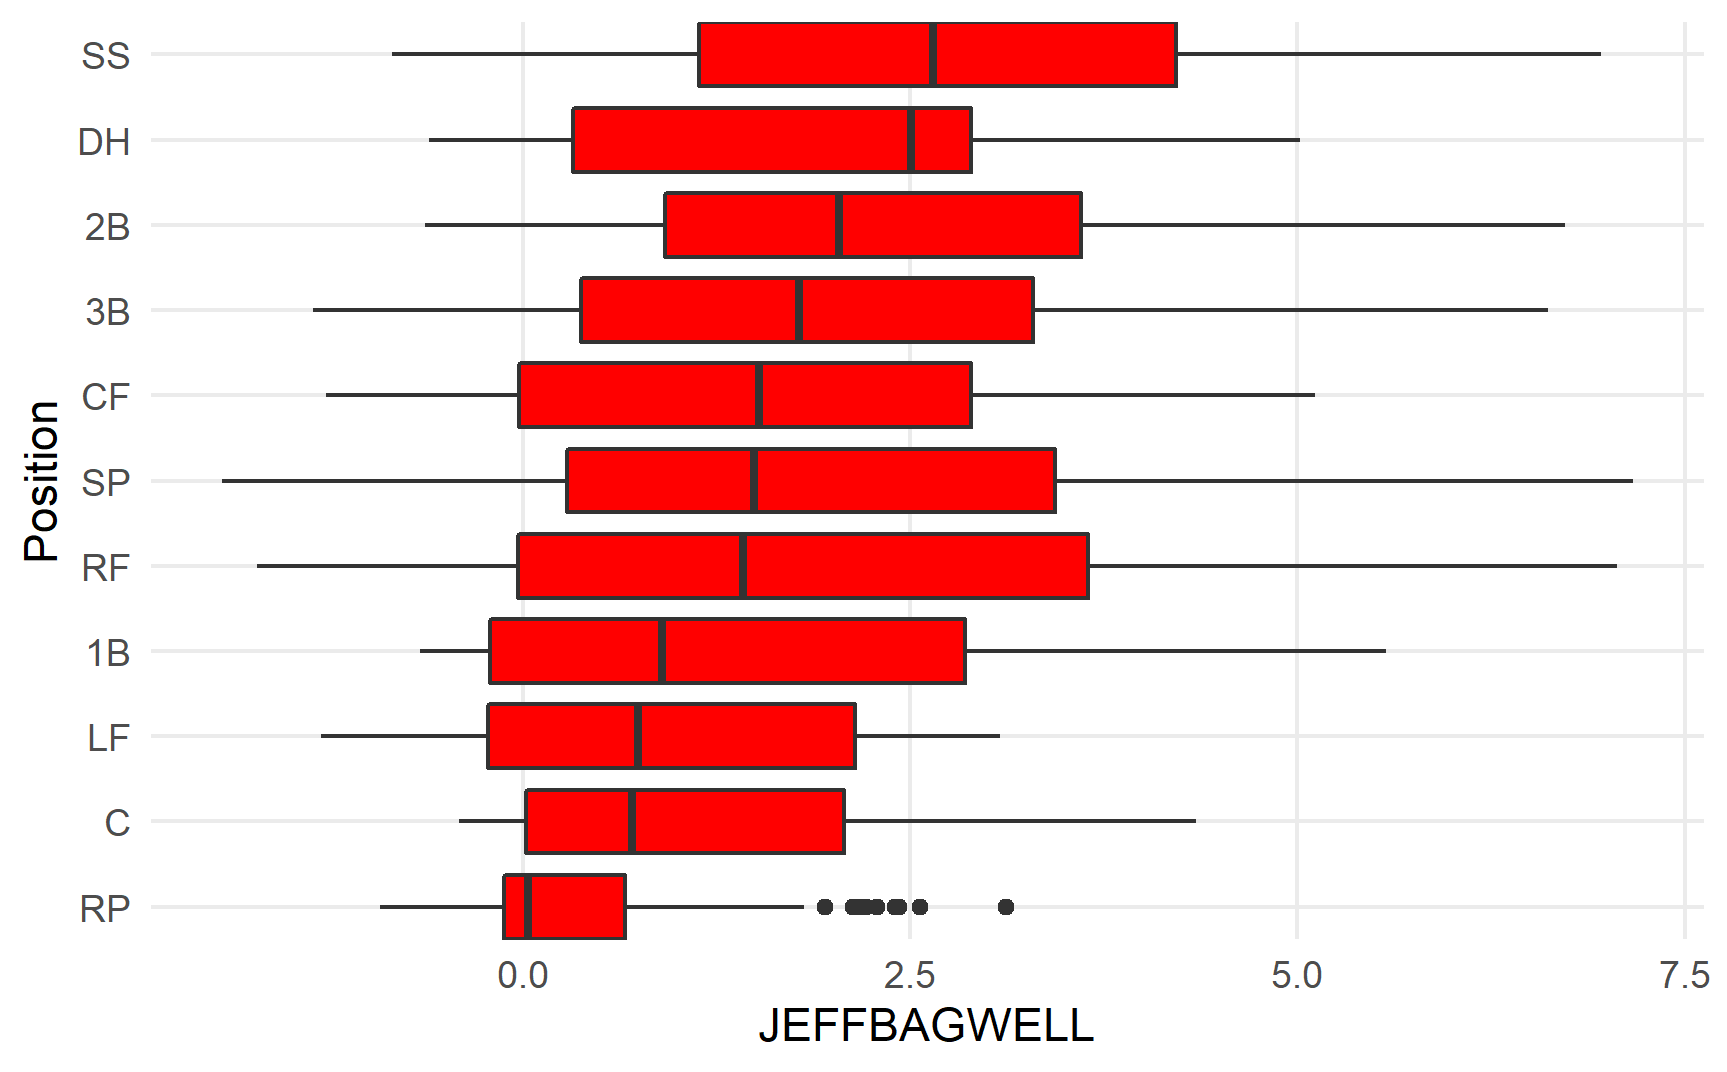
\includegraphics[width=0.7\paperwidth, scale=1.25]{war_position_boxplots.png}
\end{figure}

\subsection{Solving the Optimization Problem}

We address the discrepancy between player performance and player salary by solving a constrained optimization problem. The decision variables ($x_{i}$) are which MLB players will be selected for each team \emph{T}. $x_{i}$ is a binary variable that equals 1 if player \emph{i} is chosen, and 0 if they are not. The objective function is to maximize the JB $\forall T \in {\{1, 2, \dots,29, 30}\}$:
\begin{equation}
\sum_{i = 1}^{N} x_{i} * JB_{i}
\end{equation} where \emph{N} is the total number of eligible players in 2021 (547 players)

subject to the following constraints:

\begin{equation}
\sum_{i = 1}^{N} x_{i} = 25
\end{equation}
\begin{equation}
\sum_{i = 1}^{N} x_{i} = 5 \quad \forall x_i \in SP
\end{equation}
\begin{equation}
\sum_{i = 1}^{N} x_{i} = 7 \quad \forall x_i \in RP
\end{equation}
\begin{equation} 
\sum_{i = 1}^{N} x_{i} \geq 1 \quad \forall x_i \in CF
\end{equation}
\begin{equation} 
\sum_{i = 1}^{N} x_{i} \geq 1 \quad \forall x_i \in RF
\end{equation}
\begin{equation} 
\sum_{i = 1}^{N} x_{i} \geq 1 \quad \forall x_i \in LF
\end{equation}
\begin{equation} 
\sum_{i = 1}^{N} x_{i} \geq 1 \quad \forall x_i \in 2B
\end{equation}
\begin{equation} 
\sum_{i = 1}^{N} x_{i} \geq 1 \quad \forall x_i \in 3B
\end{equation} 
\begin{equation} 
\sum_{i = 1}^{N} x_{i} \geq 1 \quad \forall x_i \in 1B
\end{equation}
\begin{equation} 
\sum_{i = 1}^{N} x_{i} \geq 1 \quad \forall x_i \in SS
\end{equation}
\begin{equation} 
\sum_{i = 1}^{N} x_{i} = 2 \quad \forall x_i \in C
\end{equation}
\begin{equation}
\sum_{i = 1}^{N} x_{i} = 1 \quad \forall x_i \in DH
\end{equation}
\begin{equation} 
\sum_{i = 1}^{N} x_{i} = 5 \quad \forall x_i \in IF
\end{equation}
\begin{equation} 
\sum_{i = 1}^{N} x_{i}  = 5 \quad \forall x_i \in OF 
\end{equation}
\begin{equation}
\sum_{i = 1}^{N} x_{i} * x_{salary} \leq T_{salary}
\end{equation}

Equation (2) constrains each team to have exactly 25 players. Equations (3) - (15) stipulate the number of players at each position and the total number of players allowed for grouped positions.   (16) requires that each team spend no more on players than they did in the actual 2021 season. 

\section{Computational Experiment and Results}

We solve the constrained optimization problem for all 30 teams to generate each team's optimal 25 player roster. In Table 1, we see there are 5 players who are chosen for each team, and 18 players who are chosen more than 20 times. In Table 2, we see that teams have at most 3 players who were on both their actual and optimal teams. The modal amount of players to have on both the optimal and actual team is 0. 

\label{tab:teams_picked}
\begin{table}

\caption{Number of teams(max of 30) selecting player for their optimal roster}
\centering
\begin{tabular}[t]{l|r}
\hline
Player & Teams Picked\\
\hline
Darin Ruf & 30\\
\hline
Fernando Tatis Jr. & 30\\
\hline
Juan Soto & 30\\
\hline
Matt Duffy & 30\\
\hline
Matt Olson & 30\\
\hline
Shohei Ohtani & 30\\
\hline
Austin Slater & 29\\
\hline
Mike Zunino & 29\\
\hline
Jace Peterson & 28\\
\hline
Jose Ramirez & 28\\
\hline
Justin Turner & 26\\
\hline
Aaron Judge & 25\\
\hline
Carlos Correa & 25\\
\hline
Will Smith & 23\\
\hline
Andrew Albers & 22\\
\hline
Joe Ross & 22\\
\hline
Jesse Winker & 21\\
\hline
Max Fried & 21\\
\hline
Enrique Hernandez & 20\\
\hline
David Peralta & 19\\
\hline
Jacob Stallings & 18\\
\hline
Asher Wojciechowski & 17\\
\hline
German Marquez & 17\\
\hline
Brandon Lowe & 15\\
\hline
Marcus Semien & 15\\
\hline
Julio Urias & 14\\
\hline
Zack Godley & 13\\
\hline
Andy Burns & 11\\
\hline
Bryce Harper & 11\\
\hline
Scott Kazmir & 11\\
\hline
Byron Buxton & 10\\
\hline
Salvador Perez & 10\\
\hline
AJ Ramos & 8\\
\hline
Harrison Bader & 8\\
\hline
Jack Flaherty & 8\\
\hline
Joey Gallo & 7\\
\hline
AJ Pollock & 5\\
\hline
Anthony Swarzak & 5\\
\hline
Jorge Polanco & 5\\
\hline
Kyle Schwarber & 4\\
\hline
Starling Marte & 4\\
\hline
Buster Posey & 3\\
\hline
Teoscar Hernandez & 3\\
\hline
Chi Chi Gonzalez & 2\\
\hline
Jeimer Candelario & 2\\
\hline
Wade LeBlanc & 2\\
\hline
Hanser Alberto & 1\\
\hline
Jacob deGrom & 1\\
\hline
Luis Robert & 1\\
\hline
Michael A. Taylor & 1\\
\hline
\end{tabular}
\end{table}


%\begin{table}
%\caption{Number of Players who are on both the Optimal and Actual Teams}
\label{tab:optimal_and_actual}
\begin{table}

\caption{For each team, the number of players selected for their optimal team who are also on their actual team}
\centering
\begin{tabular}[t]{|>{}l|>{\centering\arraybackslash}p{10em}|}
\hline
Team & Number of Players\\
\hline
\cellcolor{gray!6}{LAD} & \cellcolor{gray!6}{3}\\
\hline
WSN & 3\\
\hline
\cellcolor{gray!6}{MIL} & \cellcolor{gray!6}{2}\\
\hline
SFG & 2\\
\hline
\cellcolor{gray!6}{TBR} & \cellcolor{gray!6}{2}\\
\hline
ATL & 1\\
\hline
\cellcolor{gray!6}{BOS} & \cellcolor{gray!6}{1}\\
\hline
CHC & 1\\
\hline
\cellcolor{gray!6}{CIN} & \cellcolor{gray!6}{1}\\
\hline
COL & 1\\
\hline
\cellcolor{gray!6}{HOU} & \cellcolor{gray!6}{1}\\
\hline
LAA & 1\\
\hline
\cellcolor{gray!6}{MIN} & \cellcolor{gray!6}{1}\\
\hline
NYY & 1\\
\hline
\cellcolor{gray!6}{OAK} & \cellcolor{gray!6}{1}\\
\hline
PHI & 1\\
\hline
\cellcolor{gray!6}{PIT} & \cellcolor{gray!6}{1}\\
\hline
SDP & 1\\
\hline
\cellcolor{gray!6}{TOR} & \cellcolor{gray!6}{1}\\
\hline
CHW & 0\\
\hline
\cellcolor{gray!6}{NYM} & \cellcolor{gray!6}{0}\\
\hline
KCR & 0\\
\hline
\cellcolor{gray!6}{STL} & \cellcolor{gray!6}{0}\\
\hline
CLE & 0\\
\hline
\cellcolor{gray!6}{MIA} & \cellcolor{gray!6}{0}\\
\hline
BAL & 0\\
\hline
\cellcolor{gray!6}{ARI} & \cellcolor{gray!6}{0}\\
\hline
SEA & 0\\
\hline
\cellcolor{gray!6}{TEX} & \cellcolor{gray!6}{0}\\
\hline
DET & 0\\
\hline
\end{tabular}
\end{table}

%\end{table}

In Figure \ref{fig:cowplot}, we sum the salary and JB for each of the actual 30 teams' rosters' in the graph on the left, and we sum the salary and JB for each of the 30 optimized teams' rosters' on the right. Each point represents a team.


\begin{figure}[h]
\caption{Scatterplots of a Team's Total JEFFBAGWELL vs. Total Dollars Spent for the Actual Team (Left)and Optimal Team (Right). The Red and Blue lines are constructed using LOESS. Note the difference in magnitude of the 2 y-axes} 
\label{fig:cowplot}
\centering
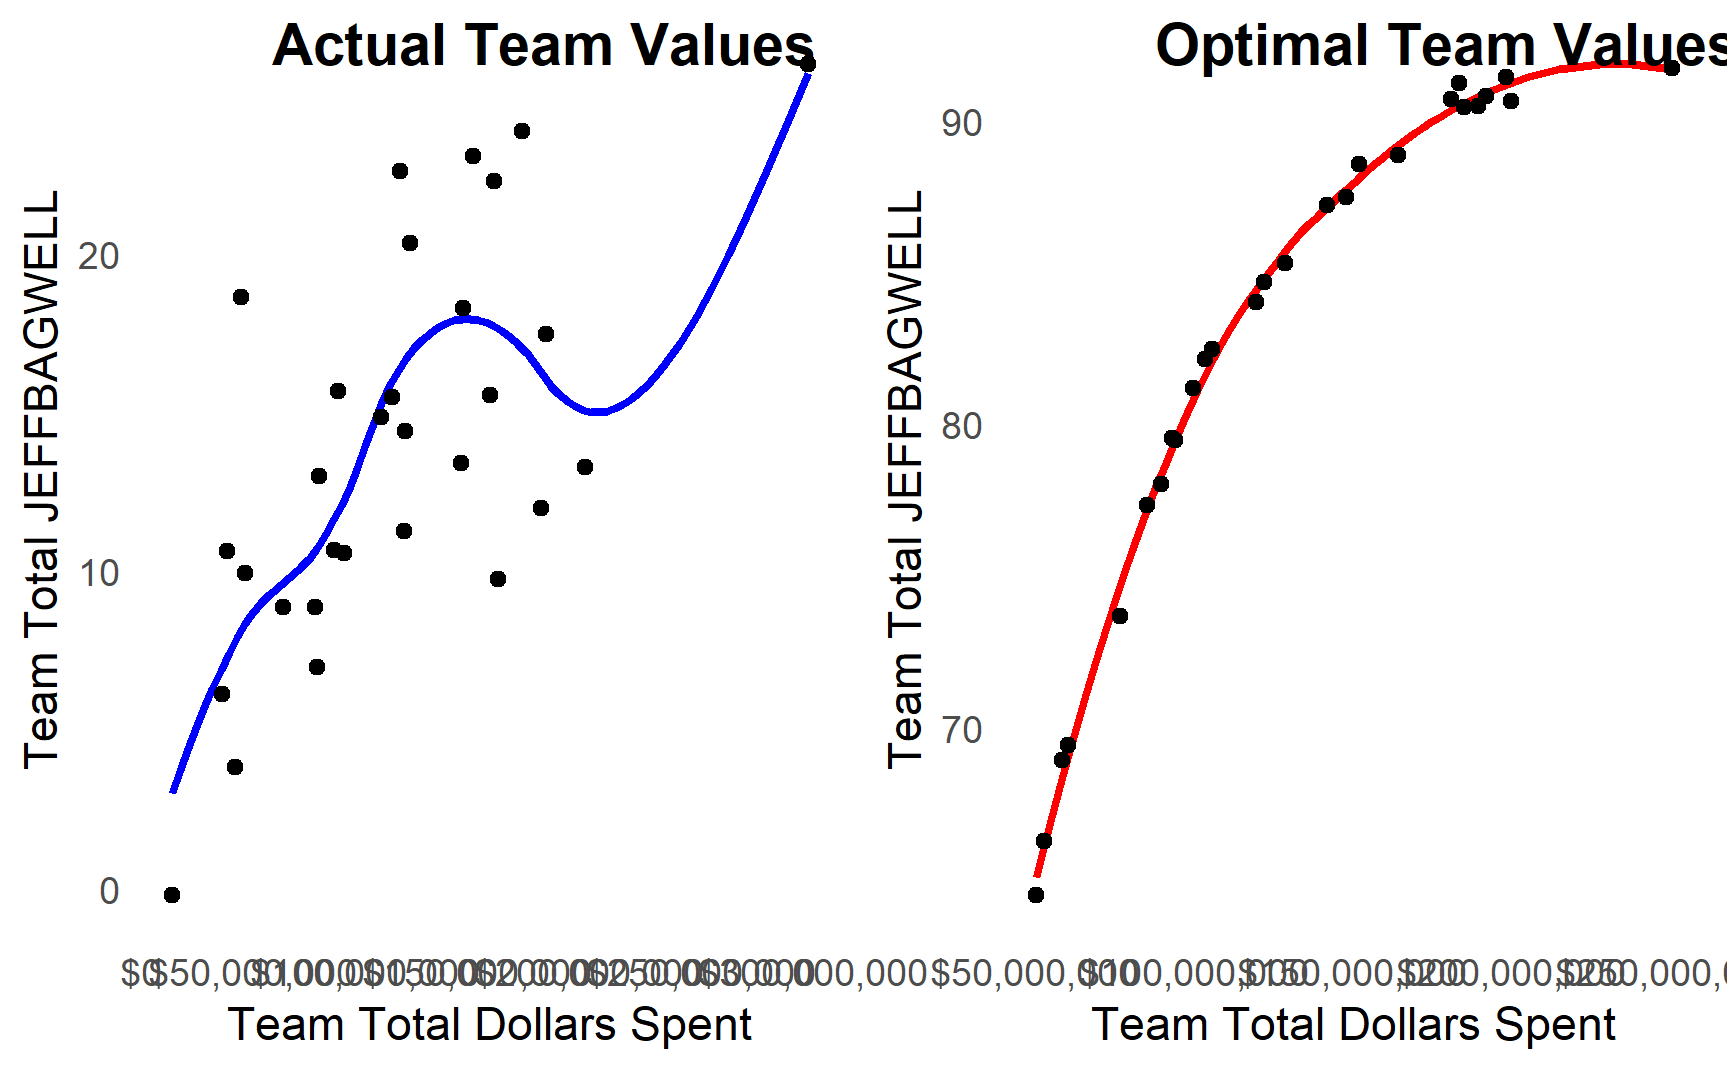
\includegraphics[width=0.7\paperwidth, scale=1.25]{bwar_salary_scatter_cowplot.png}
\end{figure}


%\begin{table}
%\caption{Five rows from the \emph{Hamilton} dataset.}
%\label{tab:example}
%\input{tables/example_raw_data.tex}
%\end{table}

\section{Discussion and Conclusions}

\subsection{Actual vs. Optimal Plots}

The shape of the two graphs in Figure \ref{fig:cowplot} is interesting. The points on the left are relatively scattered, but with a general upward trend--JB and dollars spent are positively correlated. With the smoother, we see that there is a roughly linear relationship up until the salary hits \$100,000,000. JB then \emph{decreases} up until \$150,000,000, where it then continues to increase in a concave upwards fashion.

Nearly all the points on the right fall along a single curve that is almost entirely non-decreasing, and roughly linear up until around \$200,000,000. Some takeaways from examining these two curves:
\begin{singlespace}
\begin{itemize}
	\item{The marginal value of a player is non-constant}
	\item{Almost all teams that are at the bottom of the spending distribution would benefit from spending to acquire higher JB players, but additional spending is not worthwhile for teams at the top of the distribution}
	\item{Teams can use their current status (left curve) and their optimal status (right curve) to move to a more desirable point on the JB-Salary curve}
\end{itemize}
\end{singlespace}

\subsection{Actual vs. Optimal Table}

It is surprising how few players are on the same actual and optimal team in Table 2. This table gives a rough sense of bargain star power for each team. Assuming that players are paid what they are worth (which often does not happen until free agency), the high costs of having an elite player on the team might not offset the increase in JB. Teams are able to have the most desirable combination of high JB and low cost by developing or acquiring players \emph{before} they have attained star level, since they then pay a premium once the player is an established star. 

\section{Limitations}

There are a number of limitations for this work. The metric JB is an imperfect measure of player performance. Teams know \emph{ex-ante} how much they will pay a player for the season, but they do not know what the player's performance will be prior to the season. We also use data only for the 2021 season and thus only have 30 data points for teams. It is possible that the relationship between JB and salary varies by season, and that is left as an area for future work. Furthermore, we have assumed that all players are currently available on the free agent market. This assumption is clearly unrealistic since most of the players who are selected for the optimal teams are currently under contract with particular MLB teams. 

\newpage

\bibliography{references}
\bibliographystyle{apalike}

\newpage

\section{Appendix}

\begin{figure}[h]
\caption{Histogram of Salary for Players with Salary $> \$0$}
\label{fig:salary_hist}
\centering
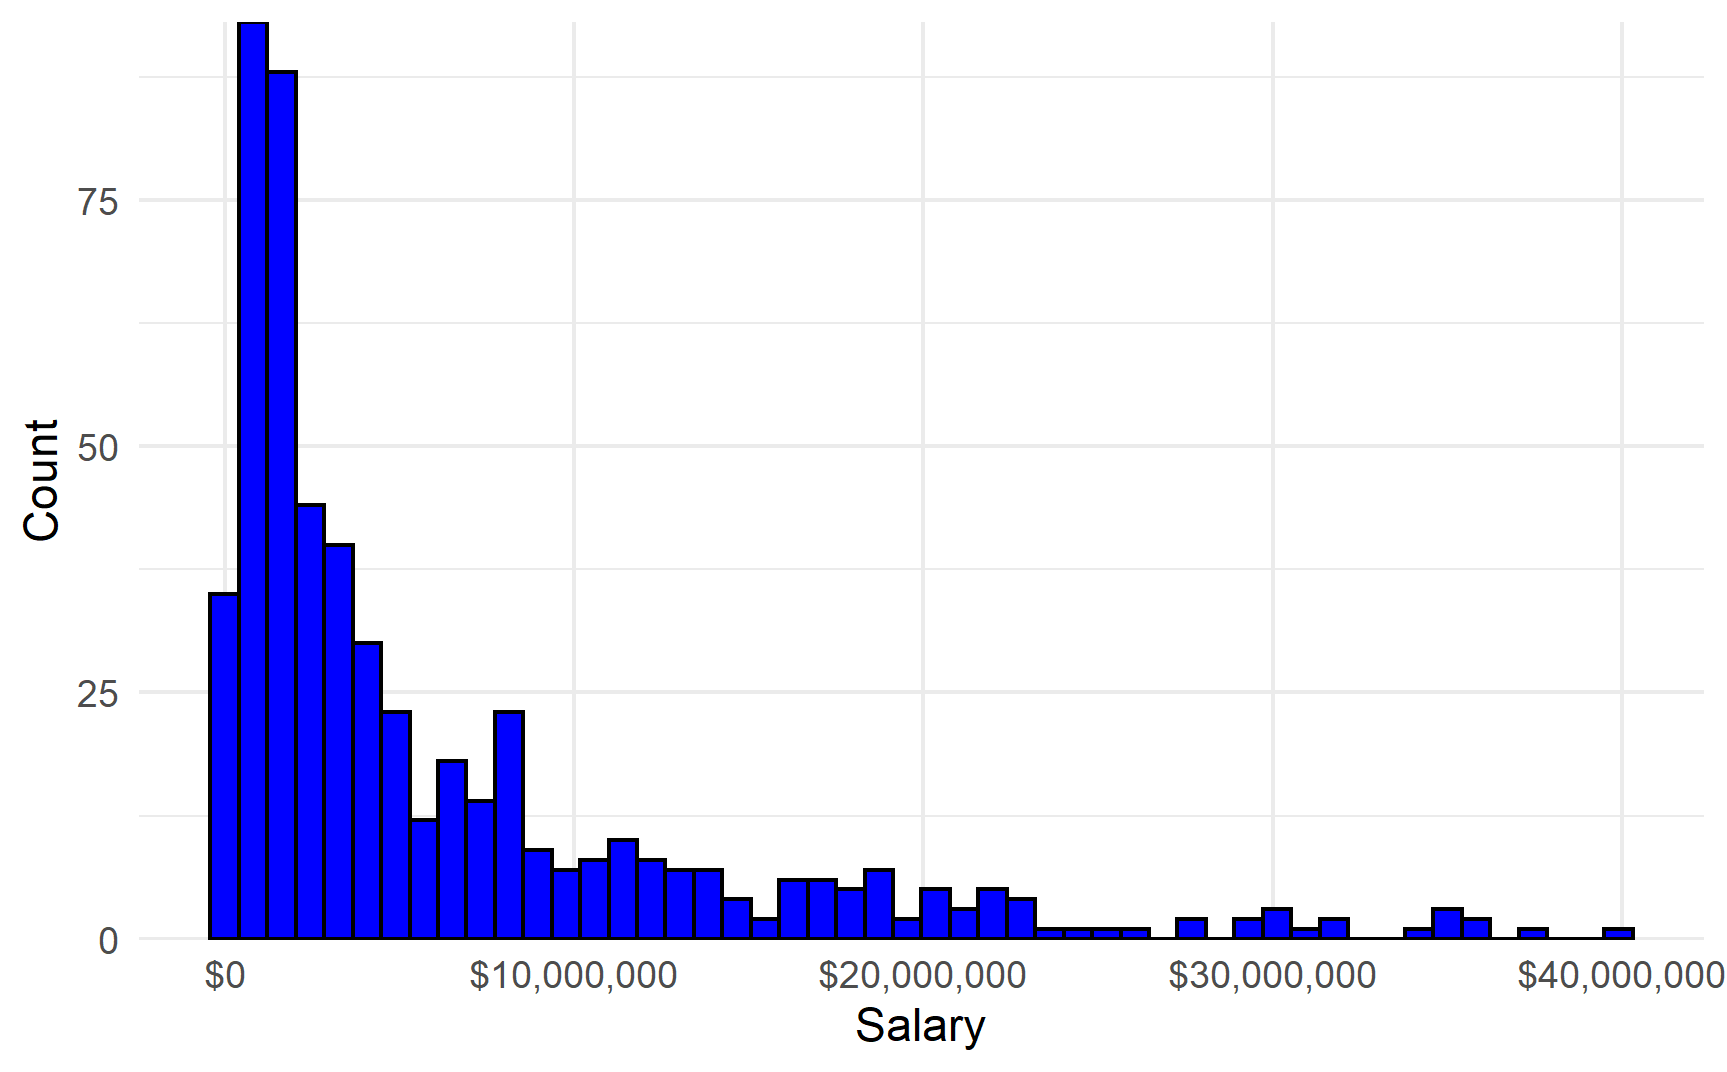
\includegraphics[width=0.7\paperwidth, scale=1.25]{salary_hist.png}
\end{figure}

\newpage
\begin{figure}[h]
\caption{Histogram of JEFFBAGWELL for Players with Salary $> \$0$}
\label{fig:bwar_hist}
\centering
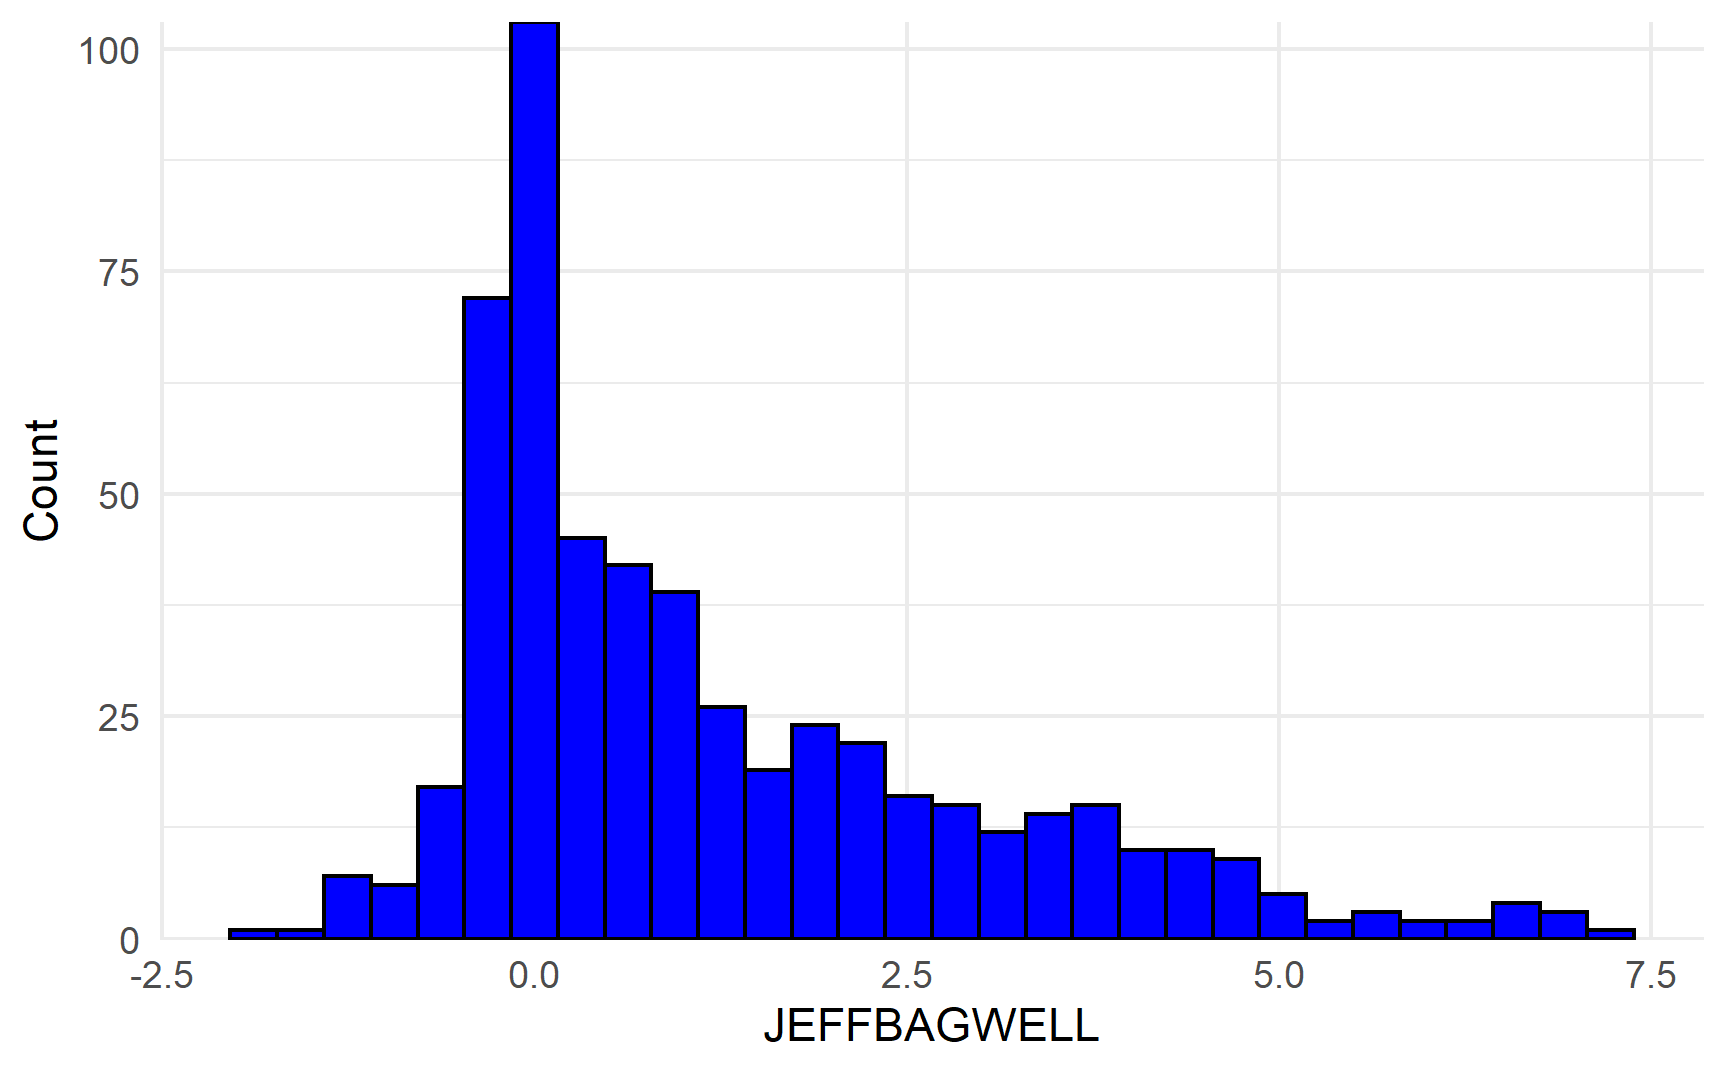
\includegraphics[width=0.7\paperwidth, scale=1.25]{war_hist.png}
\end{figure}

\end{document}